\section{Realisation}
\subsection{From Start of Realisation to 3rd March, 2018: implement first two models}
At very beginning, the first step was to attempt to implement the model of the
models including general population protocol \cite{AspnesR2007}, the network constructor \cite{MS16a} and
the terminating grid network constructor\cite{Mi17}. The first two is relatively easy because
they are much easier to be represented than the third one using widely used data structure
like adjacency list. For terminating grid network constructor, it is more complex in conception compared with
other two models. Hence it is failed to be done during this initial development period.
\paragraph{Construct software architecture}
During the development period, the most interfaces of model partition are finished according to the UML object
diagram mentioned in the \textit{design} section. An example could be the scheduler interface

\begin{lstlisting}[caption = {Interface design}, style = mykotlin]
//commit on Feb. 24th
interface Scheduler {
    fun select(population: Population): Pair<Node, Node>
}
\end{lstlisting}
\noindent
and grid network class without implementation.
\begin{lstlisting}[caption = {Grid network interface (early screenshot)}, style = mykotlin]
//commit on Feb. 24th
class NetworkConstructingPopulation constructor(scheduler: Scheduler) : LinkedPopulation {
    override val nodes: List<Node>
        get() = TODO("not implemented") //To change initializer of created properties use File | Settings | File Templates.

    override fun numOfEdge(): Int {
        TODO("not implemented") //To change body of created functions use File | Settings | File Templates.
    }

    override fun numOfNode(): Int {
        TODO("not implemented") //To change body of created functions use File | Settings | File Templates.
    }

    override fun interact(): Boolean {
        TODO("not implemented") //To change body of created functions use File | Settings | File Templates.
    }
\end{lstlisting}

\par\noindent
Though the method body not finished, these codes provides guidelines to the author for further development.
The language adopted in the project is Kotlin \cite{Kotlin}. This is A JVM language with support for pattern matching, high-order
function abstraction and operator overloading \cite{Kotlin}, which were essential characteristics for the development of this simulator.

\paragraph{Basic method for Handle centered rotation}
In the early stage, the author did aware that it would be necessary to handle centered rotation issues for terminating grid network model, hence
the author started to implement the rotation matrix, that is the equation \ref{Equ_ori}.

\begin{lstlisting}[caption = {Grid network interface (early screenshot)}, style = mykotlin]
import koma.end
import koma.extensions.get
import koma.extensions.map
import koma.mat
import koma.matrix.Matrix
import kotlin.math.roundToInt

//commit on Feb. 24th
data class LocallyCoordinatedNode(val x: Int,
                                  val y: Int,
                                  override val state: State, private val index: Int) : Node(state = state, index = index) {
    // IN-CLOCK direction rotation
    fun getLocallyRotatedNode(degree: Int): LocallyCoordinatedNode {
        val rad = degree * Math.PI / 180
        val transferMat = mat[
                Math.cos(rad), Math.sin(rad) end
                        0 - Math.sin(rad), Math.cos(rad)
                ]
        val transferred = (transferMat * mat[this.x, this.y].T).removeNegativeZeros()
        return LocallyCoordinatedNode(transferred[0, 0].roundToInt(), transferred[1, 0].roundToInt(), state, index)
    }

    private fun Matrix<Double>.removeNegativeZeros(): Matrix<Double> {
        return this.map { it -> if (it == -0.0) Math.abs(it) else it }
    }
}
\end{lstlisting}

\par\noindent
This is somehow a acceptable but naïve implementation for the only case that the rotation centre is the original point (0, 0)
and does not efficient for centred rotation involves multiple nodes needed to be rotated
(it might be optimised if taking the affine transformation form mentioned as in equation \ref{Equ_aff}).
The koma library , a scientific computing library written in Kotlin \cite{Koma}, is used here to simply the matrix calculation.
\par\noindent
Because in Kotlin, the $-0.0$ is defined as a different with $0.0$ for floating number and the value $-0.0$ is considered less than $0.0$ \cite{Kotlinfloat},
which causes issues in this calculation. Hence it is required to uniform the kind of different "$0$" using $removeNegativeZeros$ method.


\paragraph{Test-driven development}
At very first of beginning, the test codes for simple global line protocol (for testing network constructor model)
and dancing protocol (for testing general population protocol model) were written before any actual code is written. The test also included
a testing for node rotation (used later on for terminating grid network constructor). These test code written under JUnit framework \cite{JUnit}.

\par\noindent
Here is an example testing for rotation.
\begin{lstlisting}[caption = {Testing for rotation}, style = mykotlin]
//commit on Feb.24th
class LocallyCoordinatedNodeTest {

    @org.junit.Test
    fun rotationDegree() {
         // Create a node with locally coordinate (0, 0)
         val firstCase = LocallyCoordinatedNode(0, 0, State.createState(setOf("a", "b"), "a"), 1)
         // Make rotation
         val t90 = firstCase.getLocallyRotatedNode(90)
         val t180 = firstCase.getLocallyRotatedNode(180)
         val t270 = firstCase.getLocallyRotatedNode(270)
         val t360 = firstCase.getLocallyRotatedNode(360)

         assert(firstCase == t90)
         assert(firstCase == t180)
         assert(firstCase == t270)
         assert(firstCase == t360)
         // Create a node with locally coordinate (1, 1)
        `val secCase = LocallyCoordinatedNode(1, 1, State.createState(setOf("a", "b"), "a"), 1)
         //Make rotation
         val tt90 = secCase.getLocallyRotatedNode(90)
         val tt180 = secCase.getLocallyRotatedNode(180)
         val tt270 = secCase.getLocallyRotatedNode(270)
         val tt360 = secCase.getLocallyRotatedNode(360)
         assert(LocallyCoordinatedNode(1, -1, State.createState(setOf("a", "b"), "a"), 1) == tt90)
         assert(LocallyCoordinatedNode(-1, -1, State.createState(setOf("a", "b"), "a"), 1) == tt180)
         assert(LocallyCoordinatedNode(-1, 1, State.createState(setOf("a", "b"), "a"), 1) == tt270)
         assert(secCase == tt360)
    }

}
\end{lstlisting}

\subsection{From 3rd March to 26th March, 2018: Further progression}
\paragraph{Abstraction of interaction function \&\& implementation for some protocols}
During this stage, the three different interaction function concept appearing in the definition of the three models
were abstracted and represented using a Kotlin method (or say, a Kotlin function).
\begin{itemize}
  \item For general population protocol, it abstracted as
  \begin{lstlisting}[caption = {Abstraction for population protocol interaction function}, style = mykotlin]
      fun protocolFunc(initializer: ModelNode, receiver: ModelNode): Boolean
  \end{lstlisting}
   where the 1st and 2nd parameters are the two nodes selected to interact, the return value indicates whether the interaction happens ($true$ means it happens, $false$ means it not).
   \item For network constructor, it abstracted as
   \begin{lstlisting}[caption = {Abstraction for network constructor interaction function}, style = mykotlin]
      fun protocolFunc(initializer: ModelNode, receiver: ModelNode, adjacencyList: Map<ModelNode, HashSet<ModelNode>>): Pair<Boolean, Boolean>
   \end{lstlisting}
   where the 1st and 2nd parameters are the two nodes selected to interact, the 3rd parameter are the adjacency list (of which actual structure is a map) for the population that the
   first nodes located indicating the status of connection for the population. The first value in return pair indicates whether it is "effective" interaction
    (i.e. there is at least one changed state among 2 nodes and edge during the interaction, so $true$ means it is "effective", $false$ means not) while the
   second value in return pair indicates whether it is $active$ state for connection in between the two nodes after interaction($true$ means there it is active, $false$ means it is inactive).
   \item For terminating grid network, because the model is not well abstracted so it is not been abstracted successfully during this period.
\end{itemize}
\paragraph{Start of viewer implementation}
Consider the limited time for implementation, it reasonably considered as "infeasible" if building entire viewer system from sketch. The author used a dynamic
graph library called "GraphStream" \cite{GraphStream} to reduce the work amount to ensure a delivery on time.
GraphStream provides a set of basic tools for modelling dynamic graphs, such as representing elements of nodes and edges, which exactly suit for the scenario of the simulator.
\paragraph{Failed attempt to Domain Specific Language}
As initial design proposed, the author attempted to implement the functionality that allow user load their protocol from a file.
This involves loading a piece of user written code (in some Language) and then parse it into executable Kotlin code.
For time limited, it would be hard to implement a parser.
A few difficulties could be identified:
\begin{itemize}
  \item The computability of different models differs from each other. It is hard to be defined a standard set of calculation required to be supported.
  \item The form of language defined in papers requires further semantic interpretation to be transformed as executable code. A simple protocol
  sum (modulo 4) \cite{AspnesR2007} can illustrate this point. This protocol gathers the sum (modulo) of all agents to a single agent and the output
comes from the unique agent with a non-null value. The detailed rule of the protocol could be found in appendix.
Notice the rule $(v_{1}, v_{2}) \to (v_{1} + v_{2}, \bot_{v_{1} + v_{2}})$ involves an addition operation according to
the two inputs, an symbol substitution for one of output state (the second one) and a subscript addition for the second
output state. It would be a requirement to a set of powerful language grammar to define these operation if the language is required to express these operations.
\end{itemize}
A compromised but feasible solution is to utilise some language characteristics provided by Kotlin language such as operator overloading and infix expression \cite{Kotlin}.
Though defining some semantic meaning of some operations on the \textit{State} class, the transition function of sum (modulo 4) could be achieved.
Here is an implementation using this method.

\begin{lstlisting}[caption = {Implementation for transition function of sum (mod 4) protocol}, style = mykotlin]
fun sumModeFourFunc(initializer: ModelNode, receiver: ModelNode): Boolean {
    var isChanged = false
    val transferred = when{
        Pair(initializer.state,receiver.state) match Pair("[0123]","[0123]") ->{
            Pair((initializer.state + receiver.state)%4, "N" and ((initializer.state + receiver.state)%4))

        }
        Pair(initializer.state, receiver.state) match Pair("[0123]","N[0123]") -> {
            Pair(initializer.state,"N" and initializer.state)
        }

        else -> null
    }

    if (transferred!=null){
        initializer.state = transferred.first
        receiver.state = transferred.second
        isChanged = true
    }

    return isChanged
}\end{lstlisting}
\par\noindent
Note that in the implementation, there is some "new" keyword "match" and "and". The "match" keyword is used for regular expression matching,
where the first parameter before "match" keyword is the input state pair and the second parameter after this keyword is the pattern to be followed.
The "and" keyword concatenates a string and a state to produce proper results according to different situation.
\par\noindent
The \textit{initializer.state} and \textit{receiver.state} are instance of State.
The state class finally overrides (i.e. defines) 5 different binary operations including plus, minus, multiplication, division and module. The
defined operations can be modified or extended on request.

\subsection{From 27th March to 8th April, 2018: Implement terminating grid network constructor}
\paragraph{Model representation of terminating grid network constructor}
The model representation of grid network constructor has been covered in detail in the \textit{desgin} section. The
quad-direction linked structure was not initially proposed and was modified accordingly during this period of time.
The structure allow the model be modelled mathematically to follow geometrical restrictions
and limit the number of nodes connected to one nodes, which is also a limitation for this model.
\paragraph{View representation of terminating grid network constructor}
The basic concepts in the dynamic graph library, GraphStream \cite{GraphStream}, solely contains nodes, which may link to the "node (agent)" in
the three types of models to be simulated, and the edges, which may link to the "(active) connection between two nodes" for network simulator and
terminating grid network simulator. Nonetheless, there is no direct correspondence entity of "port" or "node with port" in the viewer library GraphStream.
It was required to define a node with "port" and specify what the outlook (or representation) of port.

\begin{figure}[H]
\begin{center}
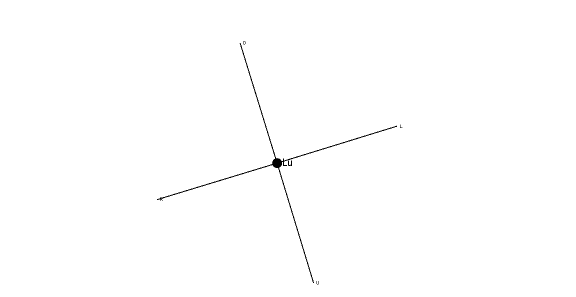
\includegraphics[width =0.7\textwidth]{context/diagram/GridNodeRepCapture.png}
\caption{Screenshot for a "node with port" in the viewer}
\label{capture_gridrep}
\end{center}
\end{figure}

\par\noindent
The figure \ref{capture_gridrep} is a typical representation of "a node with 4 ports" in terminating grid network constructor model. The centred node, which
is marked as $L_{u}$ is represented through a node representation in GraphStream. Here, to avoid any confusions, any elements including nodes and edges in
viewer part will be called as a representation while the nodes and edges in model part are still called its original name.
A port $p$ is actually another invisible node representation around the centred node $L_{u}$, and has visible line connected with $L_{u}$. Hence, a node
in terminating grid network constructor will be represented as a connected graph with 5 nodes and 4 edges in a star-like topology.

\par\noindent
Since the node representation is a graph in general, the basic manipulation of node representation in other will not suit for the node representation of
terminating grid network. Suppose there is a node representation has a real coordinate $(x_{np}, y_{np})$ (It is called "real coordinate" because the coordinate represents the true
location of the node representation and is distinct to the concept "relative coordinate" appearing in the model part.) and rotation degree $\theta_{np}$, and it intends to
another real coordinate $(x_{nq}, y_{nq})$, the movement would follows steps:
\begin{itemize}
  \item Move the centred node representation to coordinate $(x_{nq}, y_{nq})$
  \item Move the up port representation $p_{u}$ to coordinate to $(x_{nq}, y_{nq} + 1)$, right port $p_{r}$ representation to coordinate to $(x_{nq} + 1, y_{nq})$,  down port representation $p_{d}$ to coordinate to $(x_{nq}, y_{nq} - 1)$
  and left port $p_{l}$ representation to coordinate to $(x_{nq} - 1, y_{nq})$
  \item Do a centred rotation for $p_{u}$, $p_{l}$, $p_{r}$ ,$p_{d}$ regarding the centre $(x_{nq}, y_{nq})$ with rotation degree $\theta_{np}$
\end{itemize}
For rotation operation, after the centred node representation rotates, the 4 port representations are required to rotate the same degree that the centred node representation rotates.

\paragraph{Abstraction of interaction function of terminating grid network constructor}
After clarifying the model and view representation for the model, it finally could deduce the method signature for its transition function.
\begin{lstlisting}[caption = {Abstraction for terminating grid network constructor interaction function}, style = mykotlin]
  fun protocolFunc(
    firstPair: Pair<LocallyCoordinatedModelNode, Port>,
    secondPair: Pair<LocallyCoordinatedModelNode, Port>
    ): Triple<Boolean, Pair<String,String>, Boolean>
\end{lstlisting}
where the \textit{firstPair} refers the initializer node and port selected to interact and the \textit{secondPair} is the receiver.
There are three variables in the returned triple, where the first one indicates whether it is an effective interaction ($true$ if it is while $false$ for it is not), the second pair is the states
for the initializer node and receiver node respectively after the interaction, the third one indicates whether there is a "active" connection
in between two ports selected after the interaction ($true$ for there is while $false$ for there is not).

\subsection{From 9th April to 15th April, 2018: User Interface implementation and experiment}
\paragraph{Pause during simulation process and Fast-forward a simulation at initial}
The pausing function was implemented during the entire process but finishes during the final stage of implementation.
The viewer is following a "generator" pattern, which means its simulation is step based. At any time, it can stay in an intermediately
state and then resume at any time hence naturally results such a functionality.
\par\noindent
The fast-forwarding function allows user to specify a number for pre-executed selections (not number of interactions because some interactions may ineffective interactions),
and then show the results on the viewer directly after such that numbers of selections. This is normally fast then simulate in a step by step way. The key of this pattern is that
it simulates only in the model partition but does not demonstrate changes in the viewer part for initial steps, so this function will save a large amount of time from communication and synchronisation in between
model and viewer, and so from visualization animation.
\paragraph{Protocol expansibility}
Despite of the DSL was failed to be implemented, it was still possible to find some other ways to simply the process to define users' own protocols.
A possible solution might be reflection, which means “the ability of a program to manipulate as data something representing the state of the
program during its own execution" \cite{reflection96}.
\par\noindent
The simulator will check three particular classes with specific name
and check the functions and fields inside these classes that complies with some naming convention and load them if it possible when been launched each time.
More specifically, it has some classes called "protocol container", which of all implement \textit{InteractionFunctions} interface
and have their own companion object inside it. A well defined protocol $i$ contains three class static members with a same prefix, say $prefix_{i}$, in a protocol container.
The three class static members are named as "\textit{$prefix_{i}$InitialState}", "\textit{$prefix_{i}$Symbol}" and "\textit{$prefix_{i}$Func}", which are a map with String key and Int value defining the
initial configuration of the protocol, a set of String defining possible states that appearing in nodes and a function defines the transition function of a protocol.
\begin{itemize}
  \item For population protocol, the container is called \textit{PopulationProtocolFunctions}
  \item For network constructor, the container is called \textit{ShapeConstructionFunctions}
  \item For terminating grid network constructor, the container is called \textit{GridNetworkConstructingFunctions}
\end{itemize}
\par\noindent
The $prefix_{i}$ of a protocol $i$ is the "camel case" naming for the protocol and will be used in naming the protocol in user interface. For example,
a prefix "squareGridNetwork" will be presented as Square Grid Network in the simulator user interface.

\paragraph{Experiment to find ineffective protocols}
After finished the implementation of all main functionalities and built some protocols, the author examed some protocols to check their performance
and found that the dancing protocol may hard to converge under some settings. This is an evidence that the simulator is able dig into what happens inside
a protocol. A further details would be discussed later in \textit{evoluation} section.
